\documentclass[11pt]{article}
\usepackage[textwidth=18.0cm, textheight=23.0cm, top=2.0cm]{geometry}
\usepackage{pst-all}
\usepackage{amssymb}
\usepackage{tikz}
\usepackage{underscore}\begin{document}
\pagestyle{empty}


ClassName: \underline{\textbf{Class_10.2bp-42}}
\par
BinSize: \underline{\textbf{100 × 100}}
\par
ReduceSize: \underline{\textbf{100 × 100}}
\par
TypeNum: \underline{\textbf{98}}
\par
Num: \underline{\textbf{100}}
\par
OutS: \underline{\textbf{160000}}
\par
InS: \underline{\textbf{149363}}
\par
Rate: \underline{\textbf{0.934}}
\par
UB: \underline{\textbf{16}}
\par
LB0: \underline{\textbf{15}}
\par
LB: \underline{\textbf{16}}
\par
LBWithCut: \underline{\textbf{16}}
\par
NodeCut: \underline{\textbf{0}}
\par
ExtendedNodeCnt: \underline{\textbf{1}}
\par
GenNodeCnt: \underline{\textbf{1}}
\par
PrimalNode: \underline{\textbf{0}}
\par
ColumnCount: \underline{\textbf{100}}
\par
TotalCutCount: \underline{\textbf{0}}
\par
RootCutCount: \underline{\textbf{0}}
\par
LPSolverCnt: \underline{\textbf{85}}
\par
PricingSolverCnt: \underline{\textbf{85}}
\par
BranchAndBoundNum: \underline{\textbf{1}}
\par
isOpt: \underline{\textbf{false}}
\par
TimeOnInitSolution: \underline{\textbf{120.010 s}}
\par
TimeOnPrimal: \underline{\textbf{0.000 s}}
\par
TimeOnPricing: \underline{\textbf{4032.820 s}}
\par
TimeOnRmp: \underline{\textbf{0.130 s}}
\par
TotalTime: \underline{\textbf{4153.031 s}}
\par
\newpage


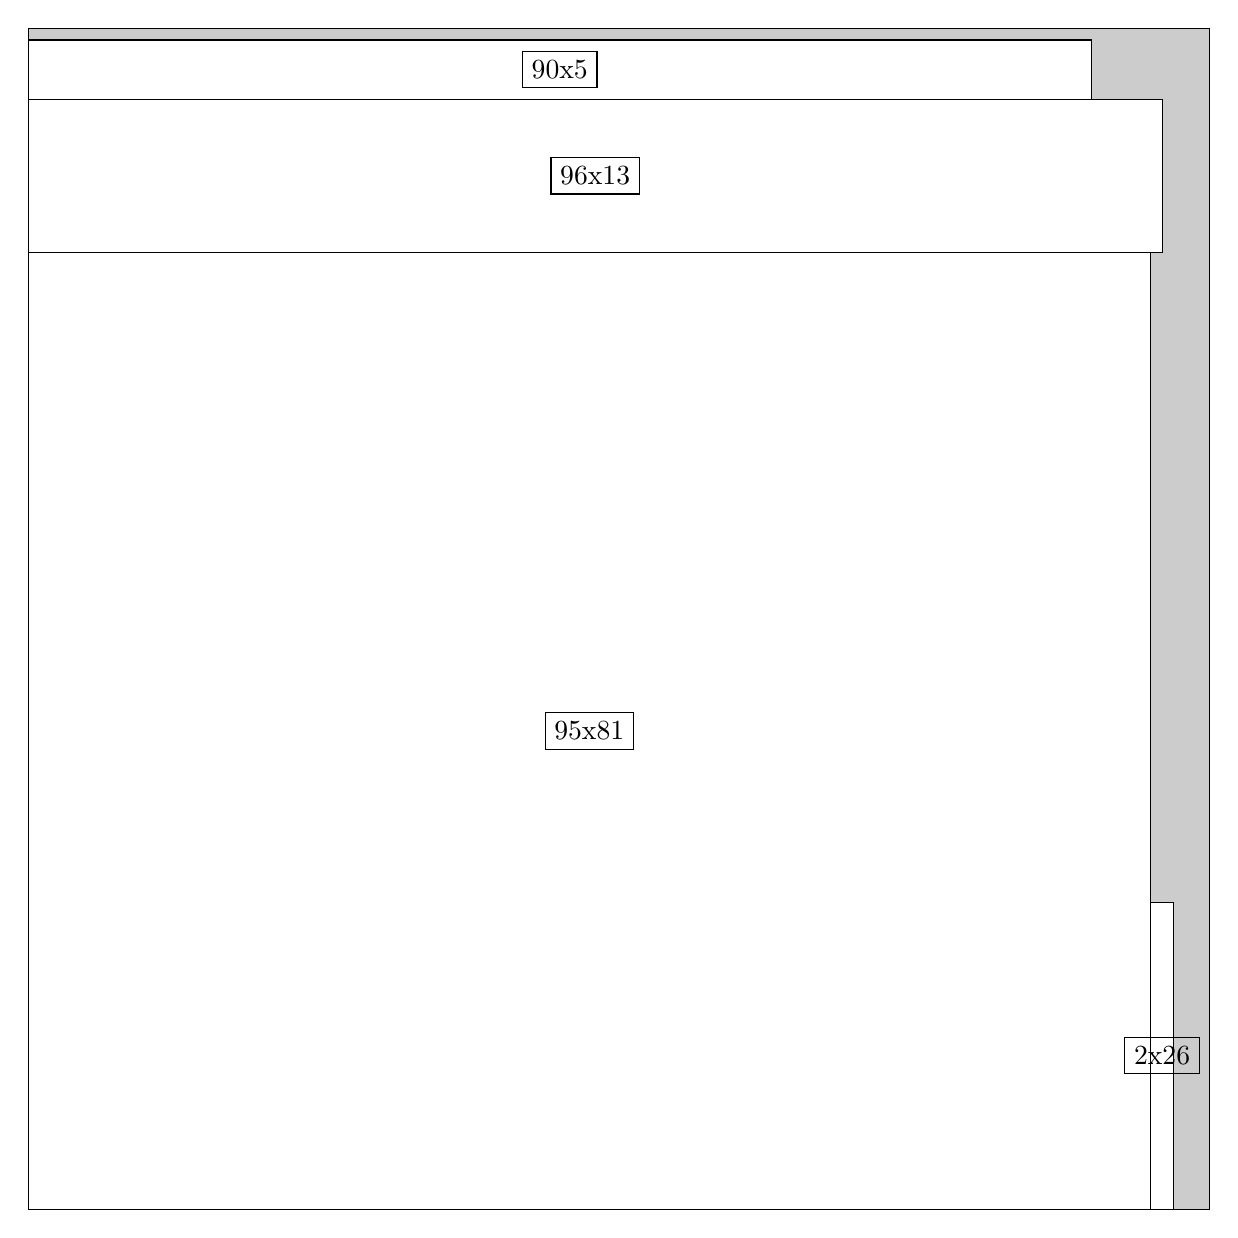
\begin{tikzpicture}[shorten >=1pt,scale=1.0,every node/.style={scale=1.0},->]
\tikzstyle{vertex}=[circle,fill=black!25,minimum size=14pt,inner sep=0pt]
\filldraw[fill=gray!40!white, draw=black] (0,0) rectangle (15.0,15.0);
\foreach \name/\x/\y/\w/\h in {96x13/0.0/12.15/14.399999999999999/1.95,95x81/0.0/0.0/14.25/12.15,90x5/0.0/14.1/13.5/0.75,2x26/14.25/0.0/0.3/3.9}
\filldraw[fill=white!40!white, draw=black] (\x,\y) rectangle node[draw] (\name) {\name} ++(\w,\h);
\end{tikzpicture}


w =96 , h =13 , x =0 , y =81 , v =1248
\par
w =95 , h =81 , x =0 , y =0 , v =7695
\par
w =90 , h =5 , x =0 , y =94 , v =450
\par
w =2 , h =26 , x =95 , y =0 , v =52
\par
\newpage


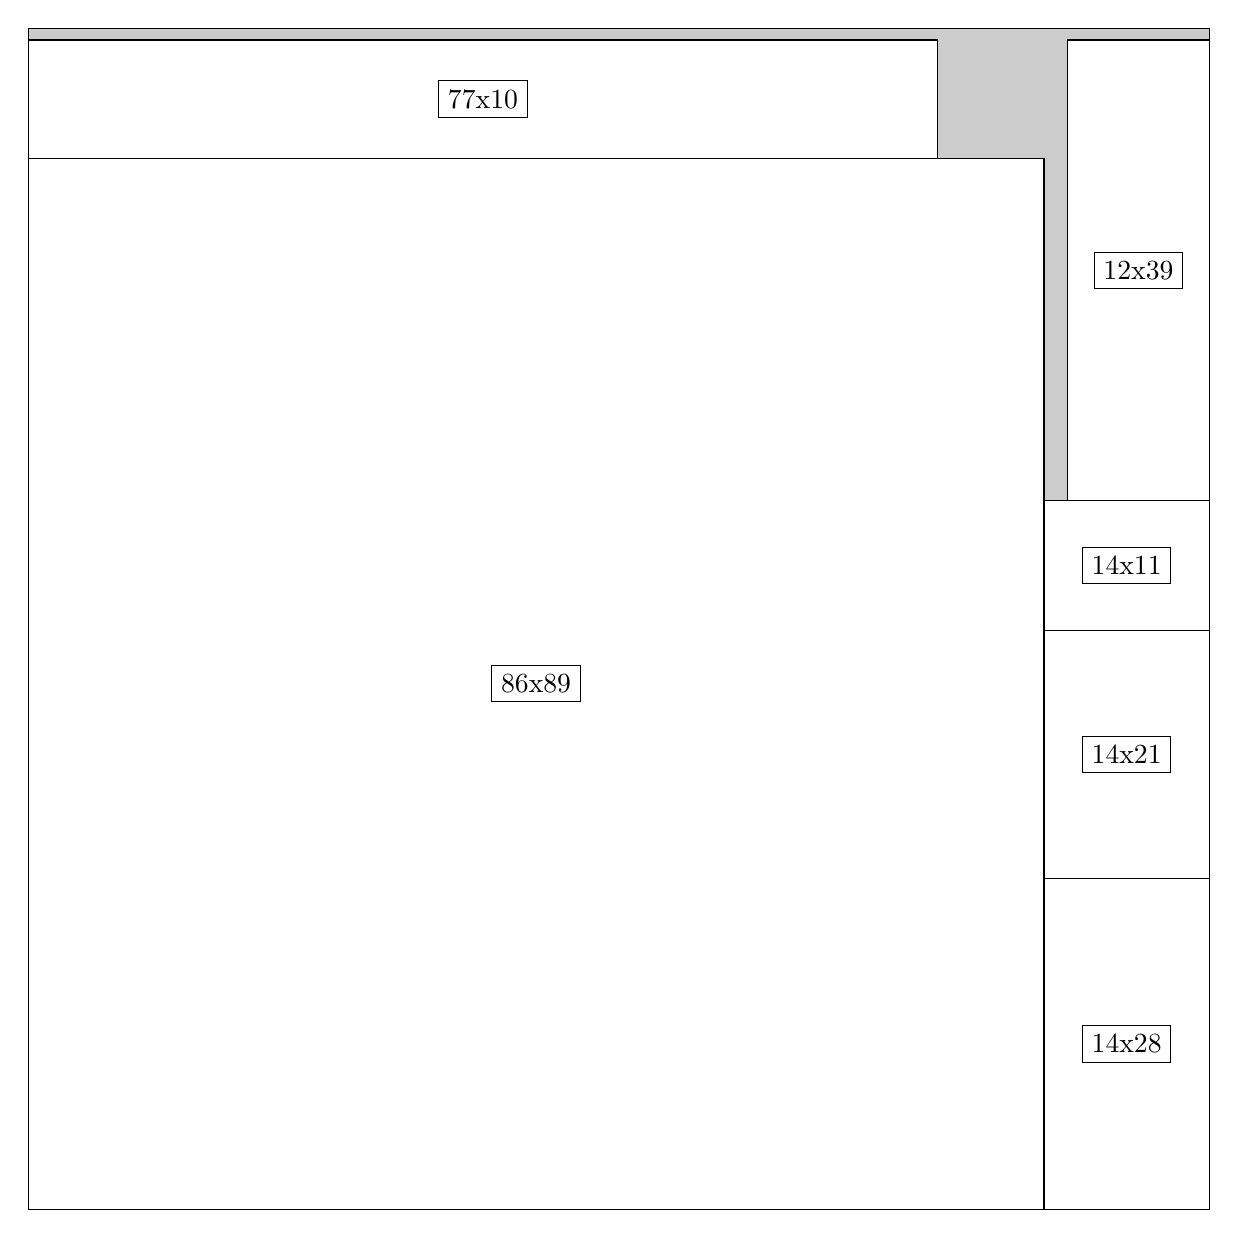
\begin{tikzpicture}[shorten >=1pt,scale=1.0,every node/.style={scale=1.0},->]
\tikzstyle{vertex}=[circle,fill=black!25,minimum size=14pt,inner sep=0pt]
\filldraw[fill=gray!40!white, draw=black] (0,0) rectangle (15.0,15.0);
\foreach \name/\x/\y/\w/\h in {86x89/0.0/0.0/12.9/13.35,77x10/0.0/13.35/11.549999999999999/1.5,12x39/13.2/9.0/1.7999999999999998/5.85,14x28/12.9/0.0/2.1/4.2,14x21/12.9/4.2/2.1/3.15,14x11/12.9/7.35/2.1/1.65}
\filldraw[fill=white!40!white, draw=black] (\x,\y) rectangle node[draw] (\name) {\name} ++(\w,\h);
\end{tikzpicture}


w =86 , h =89 , x =0 , y =0 , v =7654
\par
w =77 , h =10 , x =0 , y =89 , v =770
\par
w =12 , h =39 , x =88 , y =60 , v =468
\par
w =14 , h =28 , x =86 , y =0 , v =392
\par
w =14 , h =21 , x =86 , y =28 , v =294
\par
w =14 , h =11 , x =86 , y =49 , v =154
\par
\newpage


\begin{tikzpicture}[shorten >=1pt,scale=1.0,every node/.style={scale=1.0},->]
\tikzstyle{vertex}=[circle,fill=black!25,minimum size=14pt,inner sep=0pt]
\filldraw[fill=gray!40!white, draw=black] (0,0) rectangle (15.0,15.0);
\foreach \name/\x/\y/\w/\h in {87x86/0.0/0.0/13.049999999999999/12.9,13x94/13.049999999999999/0.0/1.95/14.1,84x13/0.0/12.9/12.6/1.95,11x6/13.35/14.1/1.65/0.8999999999999999,7x1/0.0/14.85/1.05/0.15}
\filldraw[fill=white!40!white, draw=black] (\x,\y) rectangle node[draw] (\name) {\name} ++(\w,\h);
\end{tikzpicture}


w =87 , h =86 , x =0 , y =0 , v =7482
\par
w =13 , h =94 , x =87 , y =0 , v =1222
\par
w =84 , h =13 , x =0 , y =86 , v =1092
\par
w =11 , h =6 , x =89 , y =94 , v =66
\par
w =7 , h =1 , x =0 , y =99 , v =7
\par
\newpage


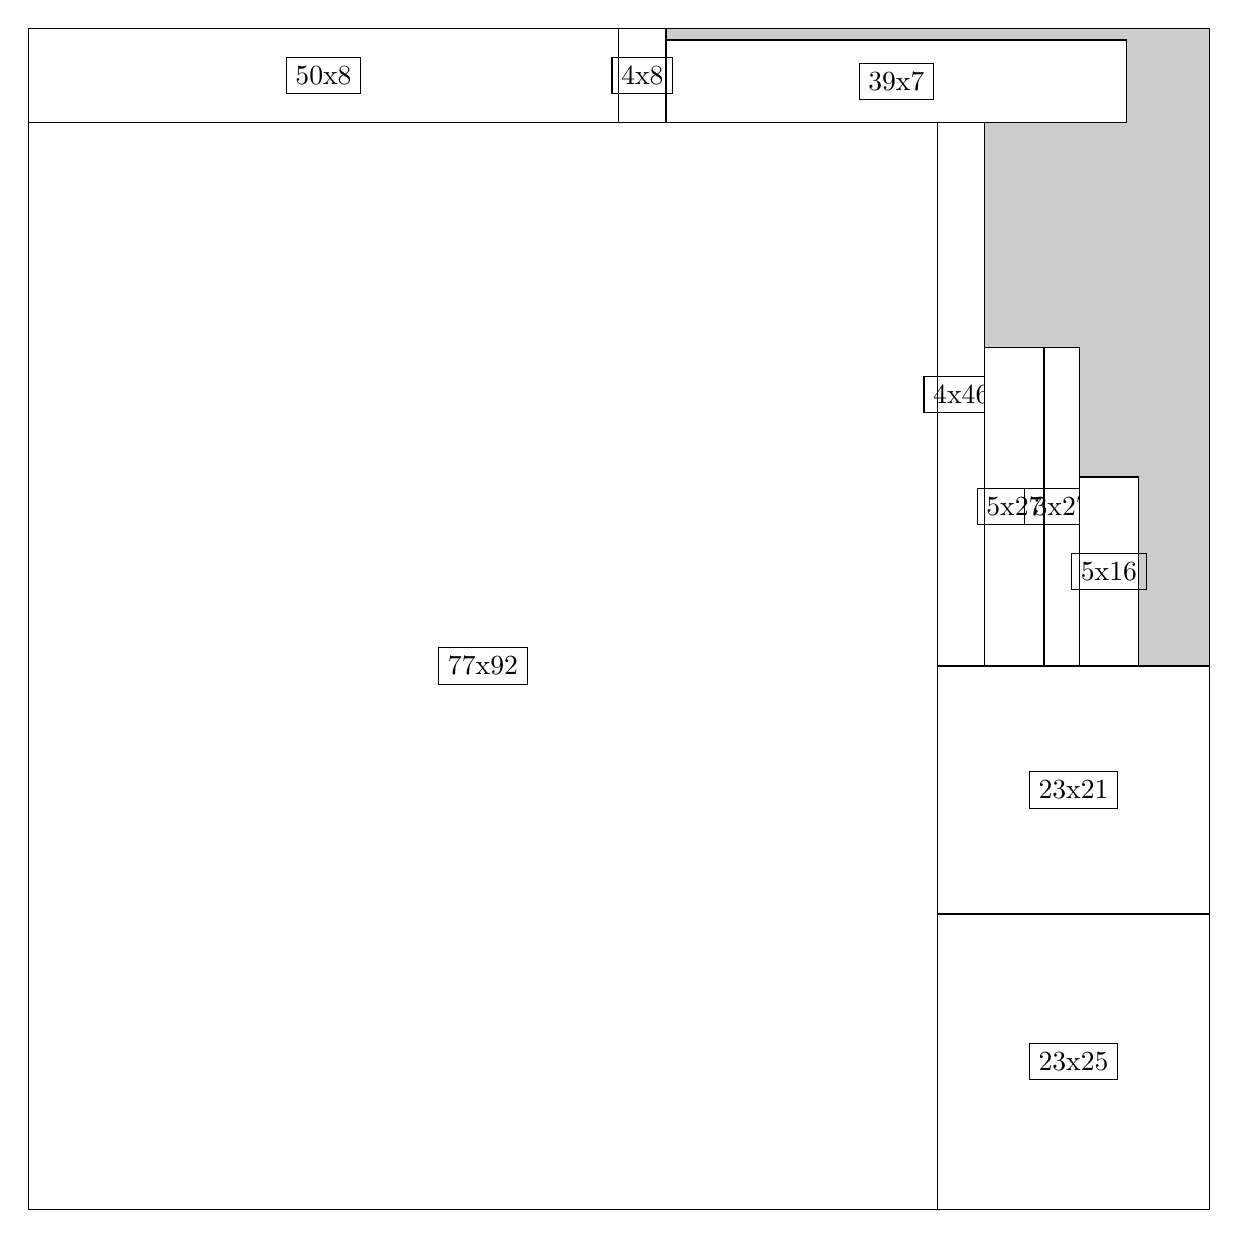
\begin{tikzpicture}[shorten >=1pt,scale=1.0,every node/.style={scale=1.0},->]
\tikzstyle{vertex}=[circle,fill=black!25,minimum size=14pt,inner sep=0pt]
\filldraw[fill=gray!40!white, draw=black] (0,0) rectangle (15.0,15.0);
\foreach \name/\x/\y/\w/\h in {77x92/0.0/0.0/11.549999999999999/13.799999999999999,23x25/11.549999999999999/0.0/3.4499999999999997/3.75,23x21/11.549999999999999/3.75/3.4499999999999997/3.15,50x8/0.0/13.799999999999999/7.5/1.2,39x7/8.1/13.799999999999999/5.85/1.05,4x46/11.549999999999999/6.8999999999999995/0.6/6.8999999999999995,5x27/12.15/6.8999999999999995/0.75/4.05,3x27/12.9/6.8999999999999995/0.44999999999999996/4.05,5x16/13.35/6.8999999999999995/0.75/2.4,4x8/7.5/13.799999999999999/0.6/1.2}
\filldraw[fill=white!40!white, draw=black] (\x,\y) rectangle node[draw] (\name) {\name} ++(\w,\h);
\end{tikzpicture}


w =77 , h =92 , x =0 , y =0 , v =7084
\par
w =23 , h =25 , x =77 , y =0 , v =575
\par
w =23 , h =21 , x =77 , y =25 , v =483
\par
w =50 , h =8 , x =0 , y =92 , v =400
\par
w =39 , h =7 , x =54 , y =92 , v =273
\par
w =4 , h =46 , x =77 , y =46 , v =184
\par
w =5 , h =27 , x =81 , y =46 , v =135
\par
w =3 , h =27 , x =86 , y =46 , v =81
\par
w =5 , h =16 , x =89 , y =46 , v =80
\par
w =4 , h =8 , x =50 , y =92 , v =32
\par
\newpage


\begin{tikzpicture}[shorten >=1pt,scale=1.0,every node/.style={scale=1.0},->]
\tikzstyle{vertex}=[circle,fill=black!25,minimum size=14pt,inner sep=0pt]
\filldraw[fill=gray!40!white, draw=black] (0,0) rectangle (15.0,15.0);
\foreach \name/\x/\y/\w/\h in {97x61/0.0/0.0/14.549999999999999/9.15,97x32/0.0/9.15/14.549999999999999/4.8,86x7/1.7999999999999998/13.95/12.9/1.05,3x79/14.549999999999999/0.0/0.44999999999999996/11.85,2x21/14.7/11.85/0.3/3.15}
\filldraw[fill=white!40!white, draw=black] (\x,\y) rectangle node[draw] (\name) {\name} ++(\w,\h);
\end{tikzpicture}


w =97 , h =61 , x =0 , y =0 , v =5917
\par
w =97 , h =32 , x =0 , y =61 , v =3104
\par
w =86 , h =7 , x =12 , y =93 , v =602
\par
w =3 , h =79 , x =97 , y =0 , v =237
\par
w =2 , h =21 , x =98 , y =79 , v =42
\par
\newpage


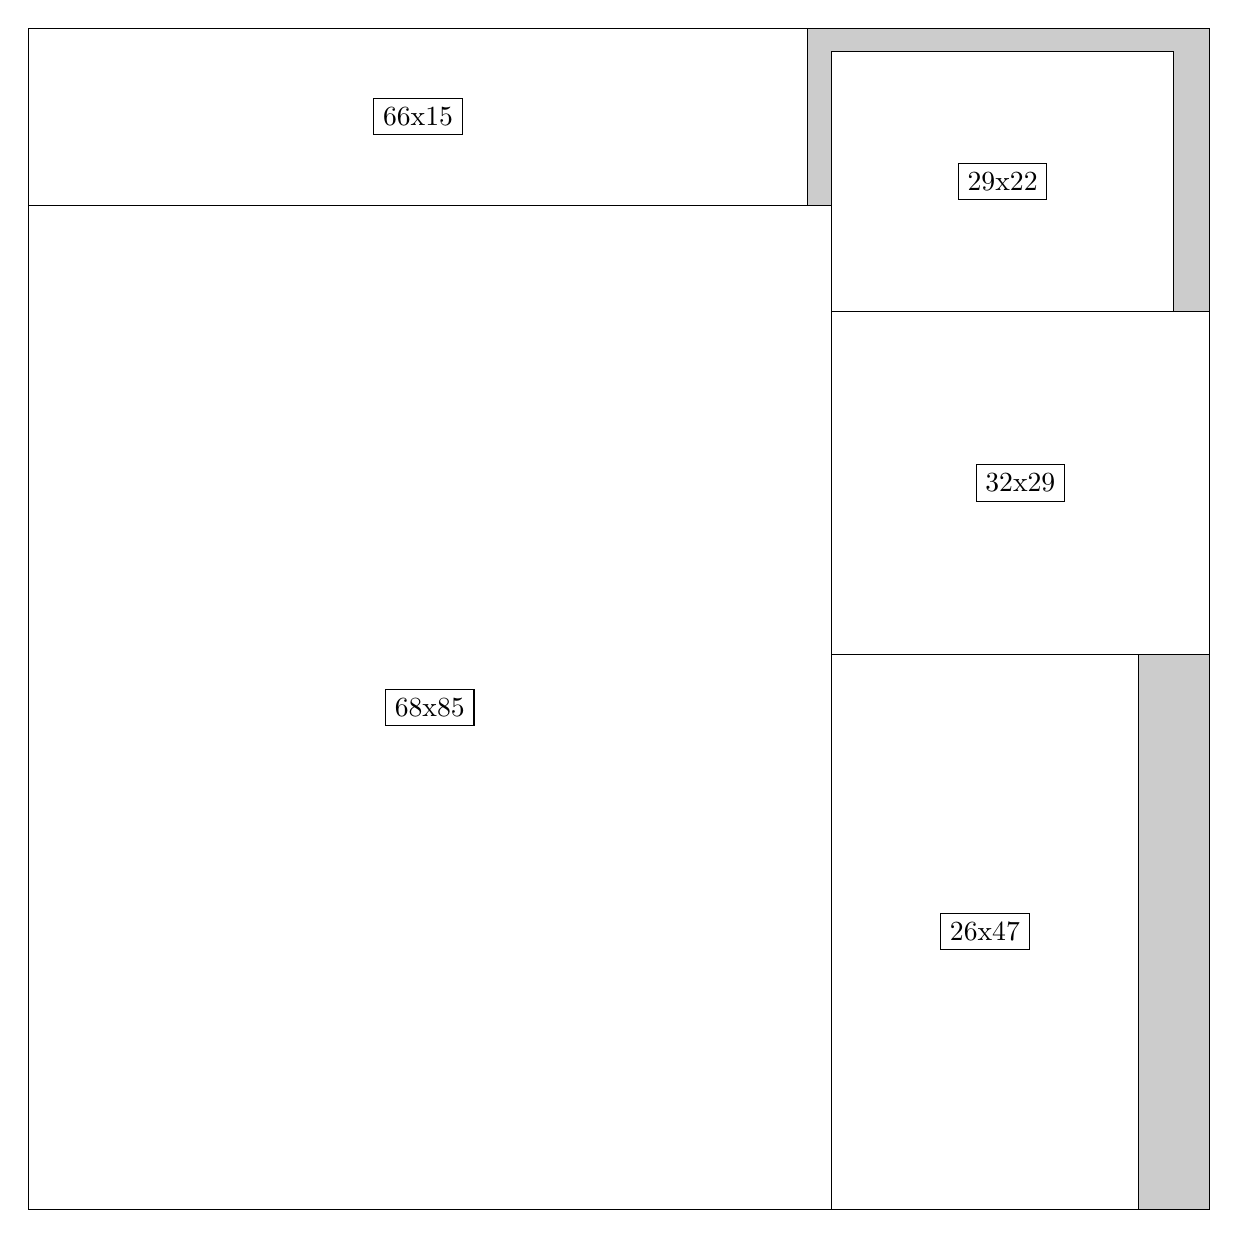
\begin{tikzpicture}[shorten >=1pt,scale=1.0,every node/.style={scale=1.0},->]
\tikzstyle{vertex}=[circle,fill=black!25,minimum size=14pt,inner sep=0pt]
\filldraw[fill=gray!40!white, draw=black] (0,0) rectangle (15.0,15.0);
\foreach \name/\x/\y/\w/\h in {68x85/0.0/0.0/10.2/12.75,26x47/10.2/0.0/3.9/7.05,66x15/0.0/12.75/9.9/2.25,32x29/10.2/7.05/4.8/4.35,29x22/10.2/11.4/4.35/3.3}
\filldraw[fill=white!40!white, draw=black] (\x,\y) rectangle node[draw] (\name) {\name} ++(\w,\h);
\end{tikzpicture}


w =68 , h =85 , x =0 , y =0 , v =5780
\par
w =26 , h =47 , x =68 , y =0 , v =1222
\par
w =66 , h =15 , x =0 , y =85 , v =990
\par
w =32 , h =29 , x =68 , y =47 , v =928
\par
w =29 , h =22 , x =68 , y =76 , v =638
\par
\newpage


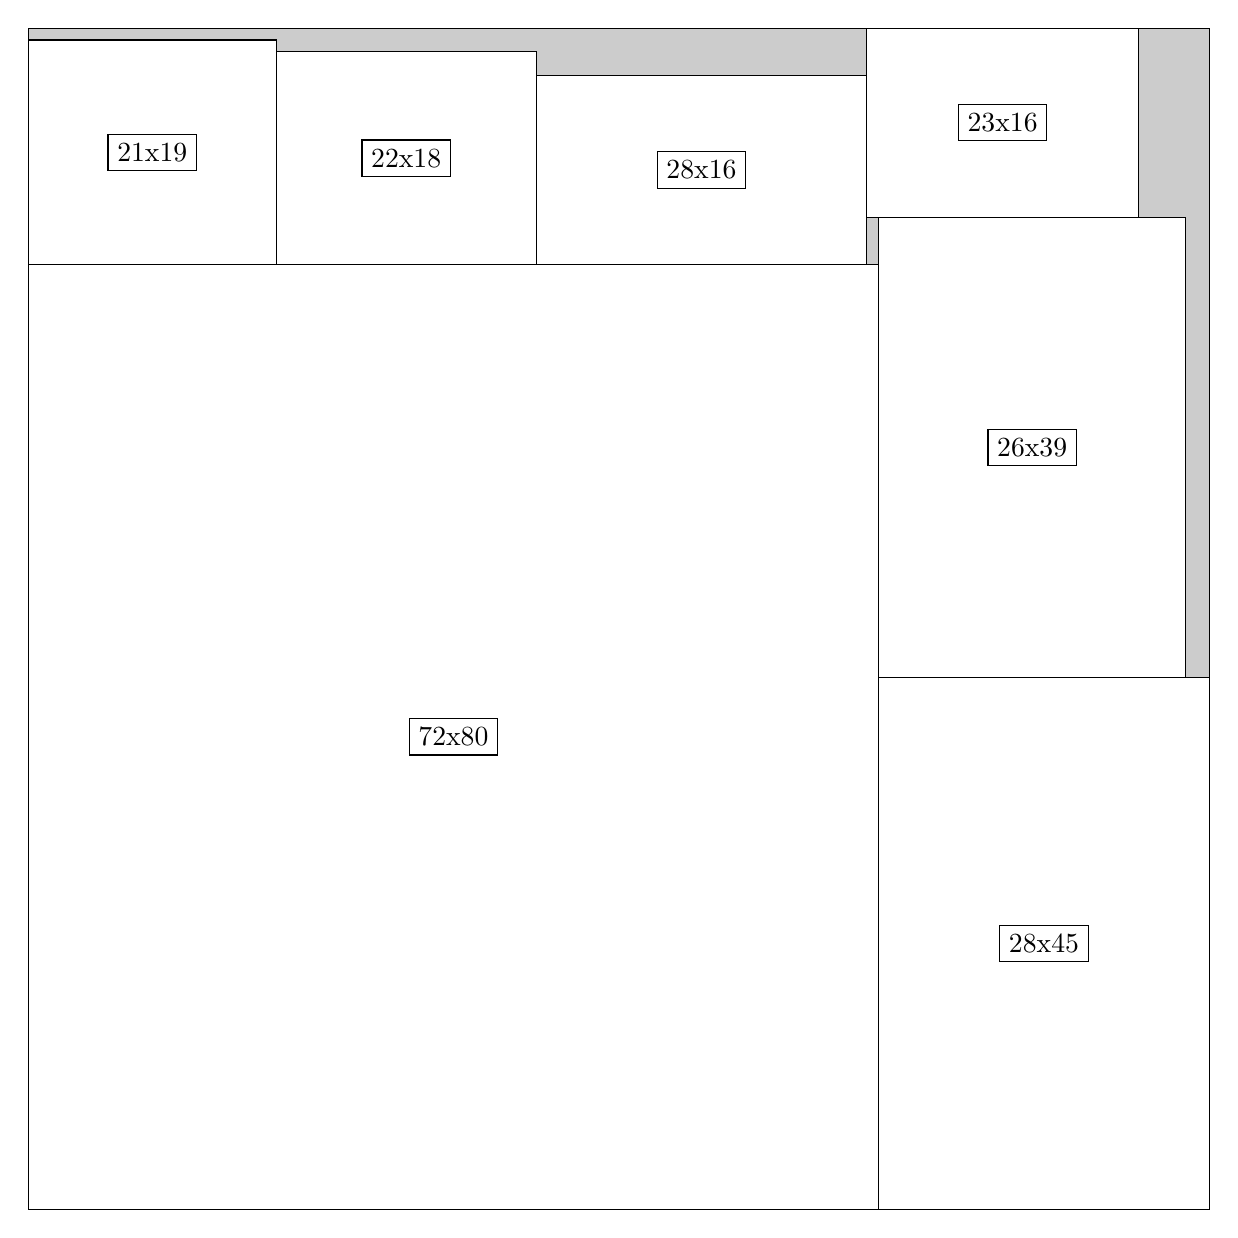
\begin{tikzpicture}[shorten >=1pt,scale=1.0,every node/.style={scale=1.0},->]
\tikzstyle{vertex}=[circle,fill=black!25,minimum size=14pt,inner sep=0pt]
\filldraw[fill=gray!40!white, draw=black] (0,0) rectangle (15.0,15.0);
\foreach \name/\x/\y/\w/\h in {72x80/0.0/0.0/10.799999999999999/12.0,26x39/10.799999999999999/6.75/3.9/5.85,28x16/6.45/12.0/4.2/2.4,21x19/0.0/12.0/3.15/2.85,22x18/3.15/12.0/3.3/2.6999999999999997,23x16/10.65/12.6/3.4499999999999997/2.4,28x45/10.799999999999999/0.0/4.2/6.75}
\filldraw[fill=white!40!white, draw=black] (\x,\y) rectangle node[draw] (\name) {\name} ++(\w,\h);
\end{tikzpicture}


w =72 , h =80 , x =0 , y =0 , v =5760
\par
w =26 , h =39 , x =72 , y =45 , v =1014
\par
w =28 , h =16 , x =43 , y =80 , v =448
\par
w =21 , h =19 , x =0 , y =80 , v =399
\par
w =22 , h =18 , x =21 , y =80 , v =396
\par
w =23 , h =16 , x =71 , y =84 , v =368
\par
w =28 , h =45 , x =72 , y =0 , v =1260
\par
\newpage


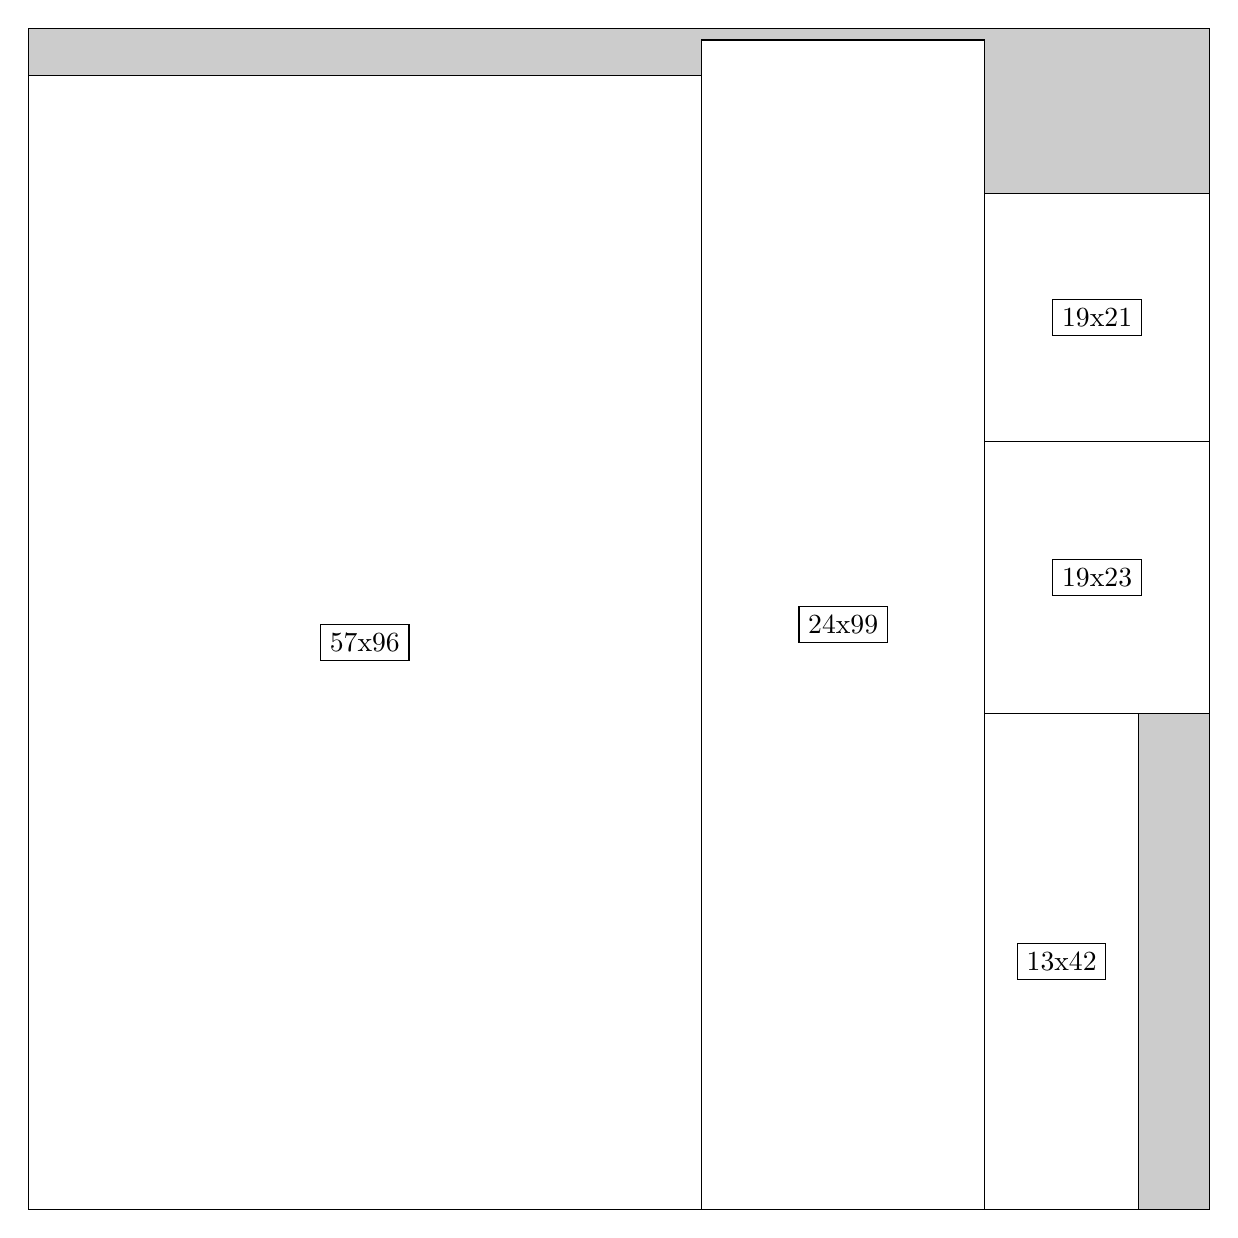
\begin{tikzpicture}[shorten >=1pt,scale=1.0,every node/.style={scale=1.0},->]
\tikzstyle{vertex}=[circle,fill=black!25,minimum size=14pt,inner sep=0pt]
\filldraw[fill=gray!40!white, draw=black] (0,0) rectangle (15.0,15.0);
\foreach \name/\x/\y/\w/\h in {57x96/0.0/0.0/8.549999999999999/14.399999999999999,24x99/8.549999999999999/0.0/3.5999999999999996/14.85,13x42/12.15/0.0/1.95/6.3,19x23/12.15/6.3/2.85/3.4499999999999997,19x21/12.15/9.75/2.85/3.15}
\filldraw[fill=white!40!white, draw=black] (\x,\y) rectangle node[draw] (\name) {\name} ++(\w,\h);
\end{tikzpicture}


w =57 , h =96 , x =0 , y =0 , v =5472
\par
w =24 , h =99 , x =57 , y =0 , v =2376
\par
w =13 , h =42 , x =81 , y =0 , v =546
\par
w =19 , h =23 , x =81 , y =42 , v =437
\par
w =19 , h =21 , x =81 , y =65 , v =399
\par
\newpage


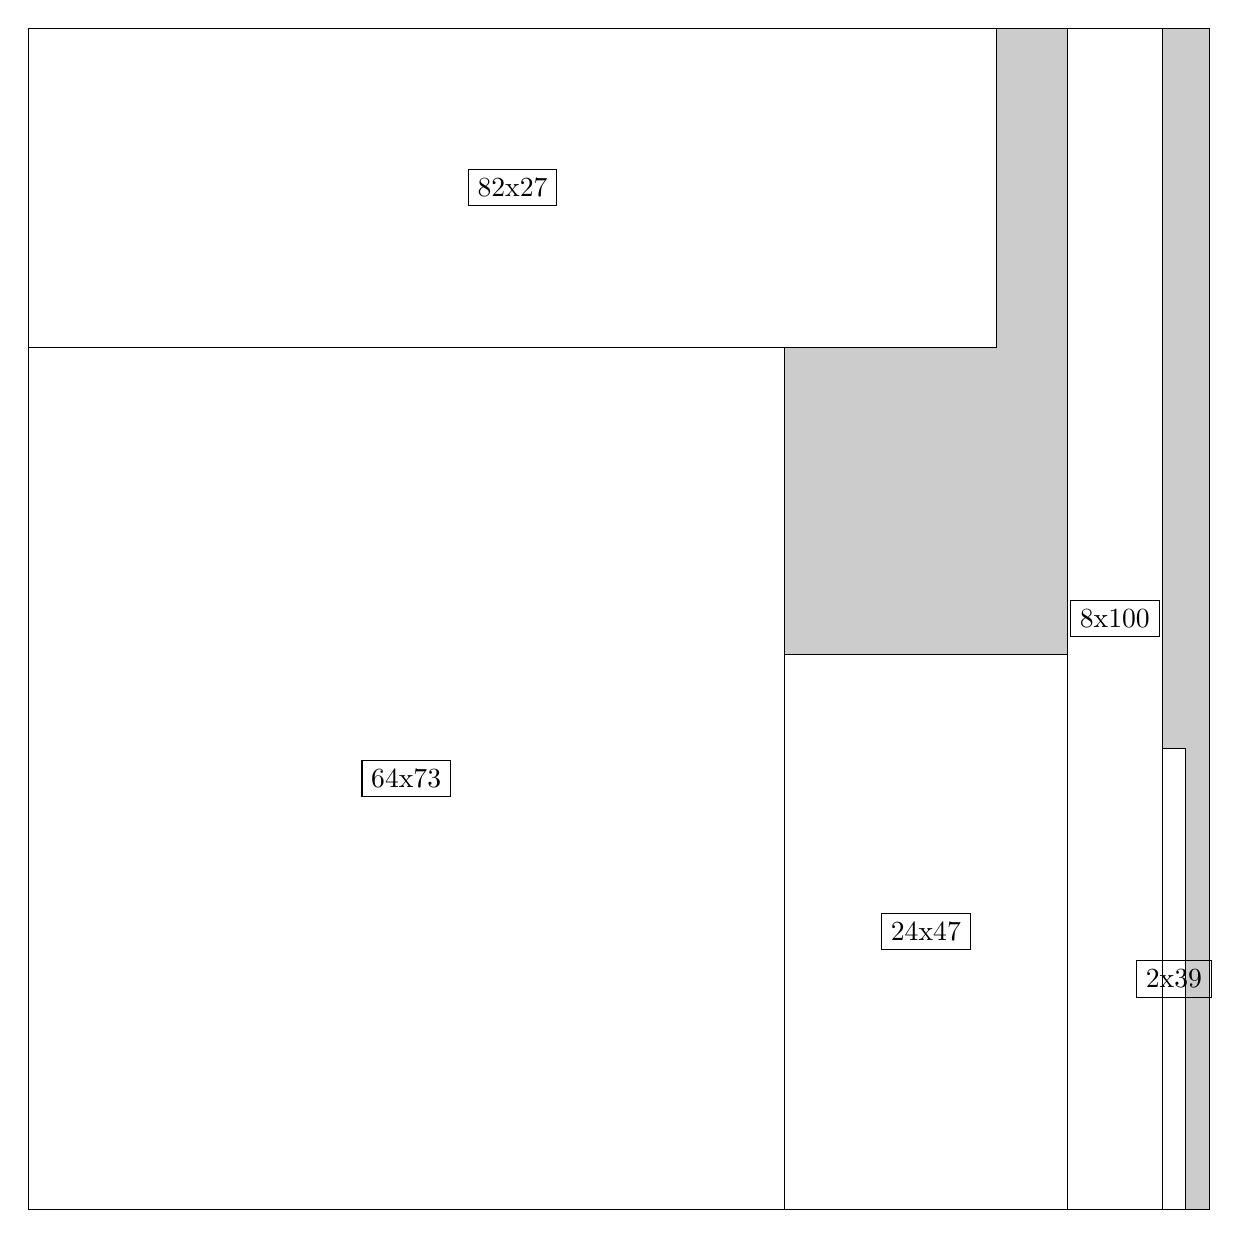
\begin{tikzpicture}[shorten >=1pt,scale=1.0,every node/.style={scale=1.0},->]
\tikzstyle{vertex}=[circle,fill=black!25,minimum size=14pt,inner sep=0pt]
\filldraw[fill=gray!40!white, draw=black] (0,0) rectangle (15.0,15.0);
\foreach \name/\x/\y/\w/\h in {64x73/0.0/0.0/9.6/10.95,82x27/0.0/10.95/12.299999999999999/4.05,24x47/9.6/0.0/3.5999999999999996/7.05,8x100/13.2/0.0/1.2/15.0,2x39/14.399999999999999/0.0/0.3/5.85}
\filldraw[fill=white!40!white, draw=black] (\x,\y) rectangle node[draw] (\name) {\name} ++(\w,\h);
\end{tikzpicture}


w =64 , h =73 , x =0 , y =0 , v =4672
\par
w =82 , h =27 , x =0 , y =73 , v =2214
\par
w =24 , h =47 , x =64 , y =0 , v =1128
\par
w =8 , h =100 , x =88 , y =0 , v =800
\par
w =2 , h =39 , x =96 , y =0 , v =78
\par
\newpage


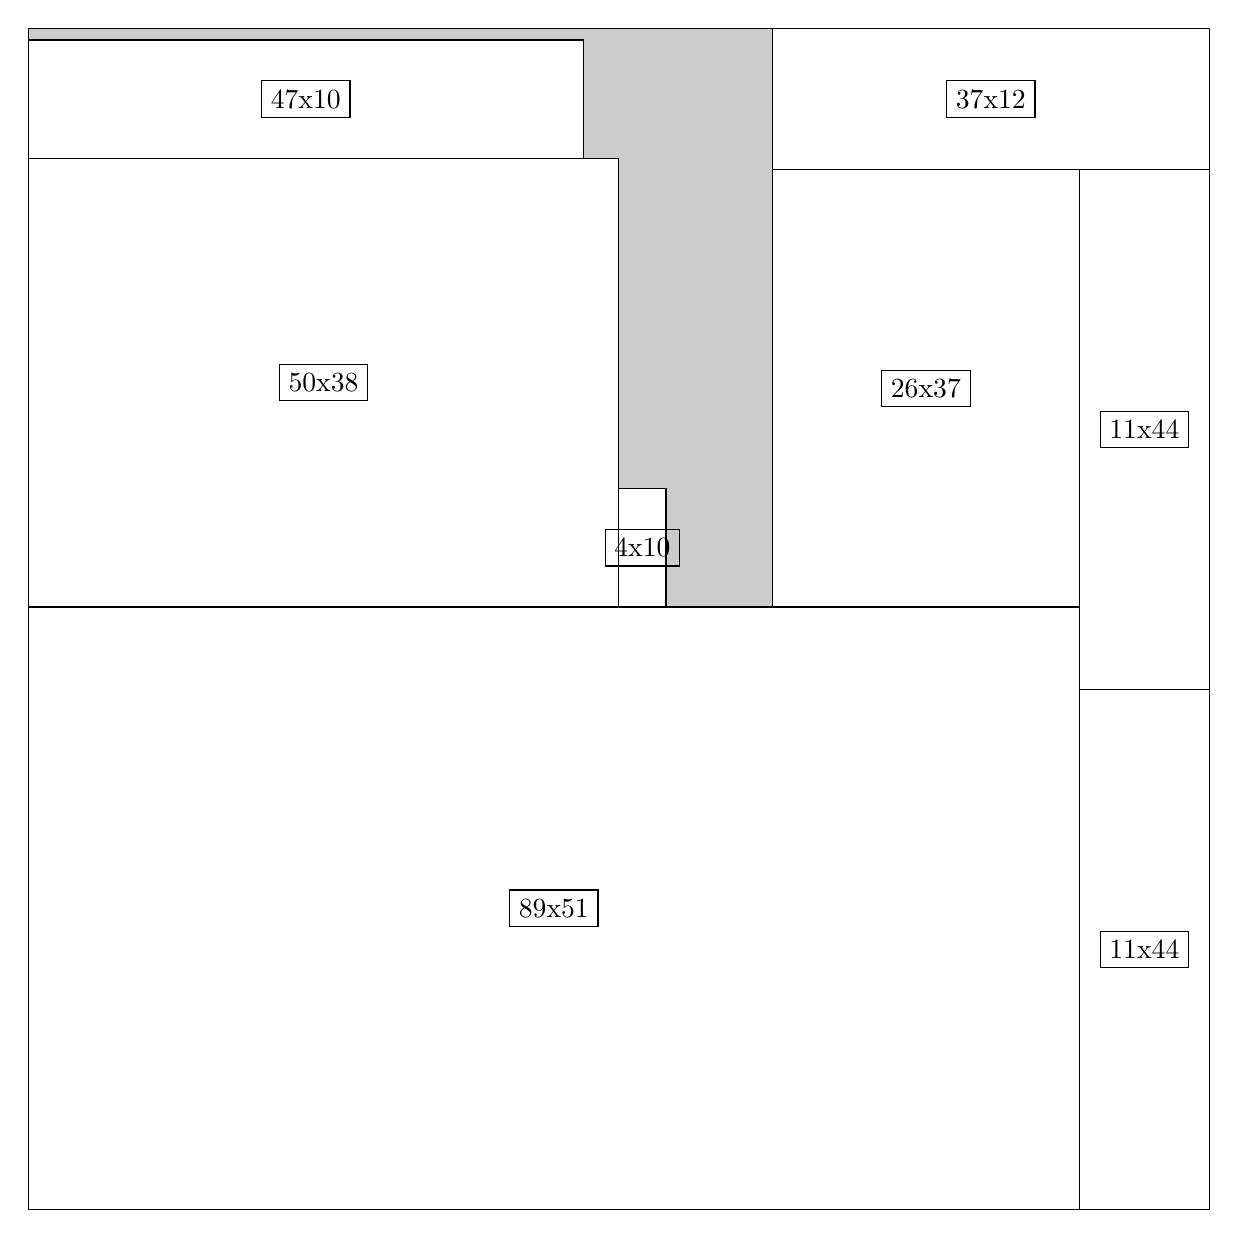
\begin{tikzpicture}[shorten >=1pt,scale=1.0,every node/.style={scale=1.0},->]
\tikzstyle{vertex}=[circle,fill=black!25,minimum size=14pt,inner sep=0pt]
\filldraw[fill=gray!40!white, draw=black] (0,0) rectangle (15.0,15.0);
\foreach \name/\x/\y/\w/\h in {89x51/0.0/0.0/13.35/7.6499999999999995,50x38/0.0/7.6499999999999995/7.5/5.7,26x37/9.45/7.6499999999999995/3.9/5.55,11x44/13.35/0.0/1.65/6.6,11x44/13.35/6.6/1.65/6.6,47x10/0.0/13.35/7.05/1.5,37x12/9.45/13.2/5.55/1.7999999999999998,4x10/7.5/7.6499999999999995/0.6/1.5}
\filldraw[fill=white!40!white, draw=black] (\x,\y) rectangle node[draw] (\name) {\name} ++(\w,\h);
\end{tikzpicture}


w =89 , h =51 , x =0 , y =0 , v =4539
\par
w =50 , h =38 , x =0 , y =51 , v =1900
\par
w =26 , h =37 , x =63 , y =51 , v =962
\par
w =11 , h =44 , x =89 , y =0 , v =484
\par
w =11 , h =44 , x =89 , y =44 , v =484
\par
w =47 , h =10 , x =0 , y =89 , v =470
\par
w =37 , h =12 , x =63 , y =88 , v =444
\par
w =4 , h =10 , x =50 , y =51 , v =40
\par
\newpage


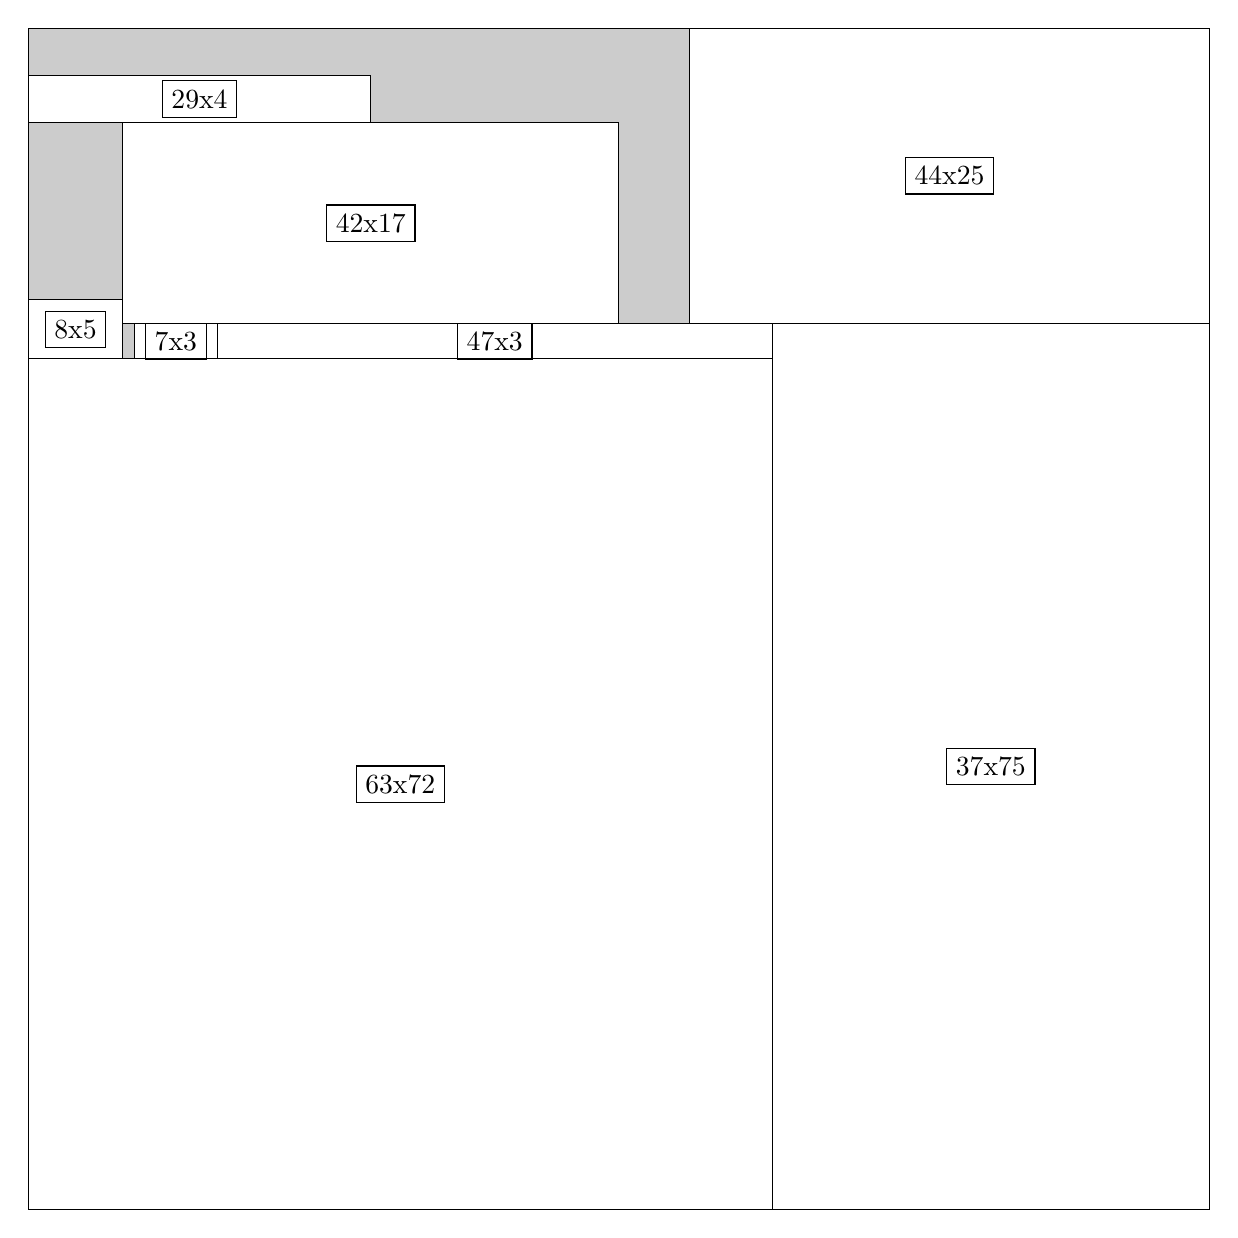
\begin{tikzpicture}[shorten >=1pt,scale=1.0,every node/.style={scale=1.0},->]
\tikzstyle{vertex}=[circle,fill=black!25,minimum size=14pt,inner sep=0pt]
\filldraw[fill=gray!40!white, draw=black] (0,0) rectangle (15.0,15.0);
\foreach \name/\x/\y/\w/\h in {63x72/0.0/0.0/9.45/10.799999999999999,37x75/9.45/0.0/5.55/11.25,44x25/8.4/11.25/6.6/3.75,42x17/1.2/11.25/6.3/2.55,47x3/2.4/10.799999999999999/7.05/0.44999999999999996,29x4/0.0/13.799999999999999/4.35/0.6,8x5/0.0/10.799999999999999/1.2/0.75,7x3/1.3499999999999999/10.799999999999999/1.05/0.44999999999999996}
\filldraw[fill=white!40!white, draw=black] (\x,\y) rectangle node[draw] (\name) {\name} ++(\w,\h);
\end{tikzpicture}


w =63 , h =72 , x =0 , y =0 , v =4536
\par
w =37 , h =75 , x =63 , y =0 , v =2775
\par
w =44 , h =25 , x =56 , y =75 , v =1100
\par
w =42 , h =17 , x =8 , y =75 , v =714
\par
w =47 , h =3 , x =16 , y =72 , v =141
\par
w =29 , h =4 , x =0 , y =92 , v =116
\par
w =8 , h =5 , x =0 , y =72 , v =40
\par
w =7 , h =3 , x =9 , y =72 , v =21
\par
\newpage


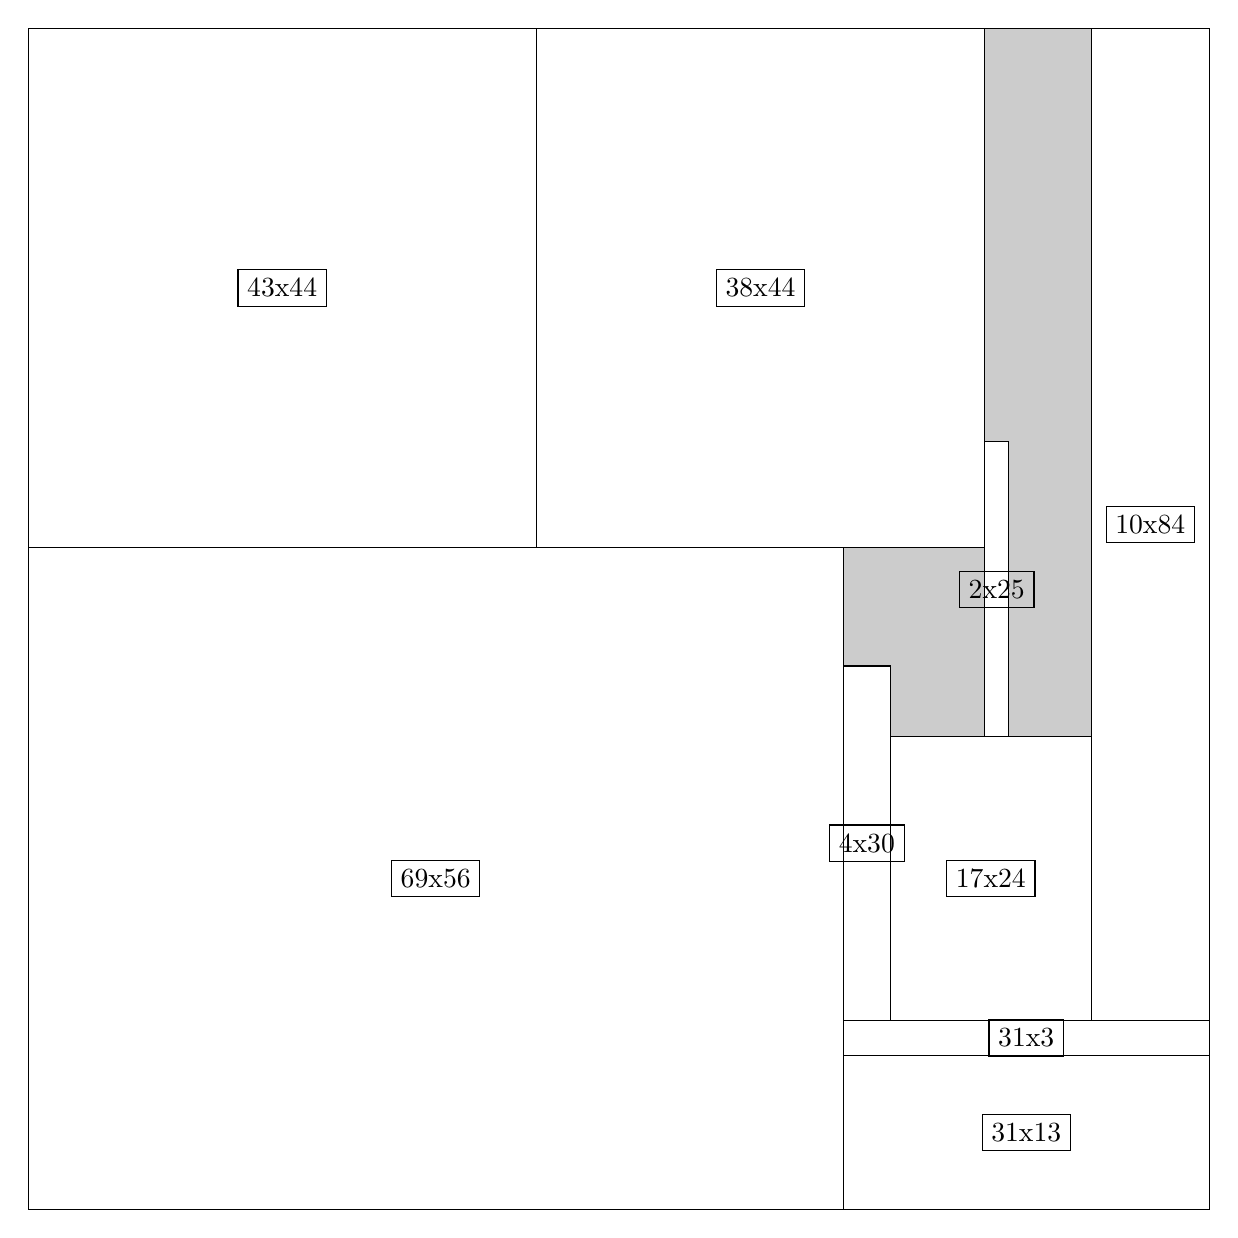
\begin{tikzpicture}[shorten >=1pt,scale=1.0,every node/.style={scale=1.0},->]
\tikzstyle{vertex}=[circle,fill=black!25,minimum size=14pt,inner sep=0pt]
\filldraw[fill=gray!40!white, draw=black] (0,0) rectangle (15.0,15.0);
\foreach \name/\x/\y/\w/\h in {69x56/0.0/0.0/10.35/8.4,43x44/0.0/8.4/6.45/6.6,38x44/6.45/8.4/5.7/6.6,10x84/13.5/2.4/1.5/12.6,17x24/10.95/2.4/2.55/3.5999999999999996,31x13/10.35/0.0/4.6499999999999995/1.95,4x30/10.35/2.4/0.6/4.5,31x3/10.35/1.95/4.6499999999999995/0.44999999999999996,2x25/12.15/6.0/0.3/3.75}
\filldraw[fill=white!40!white, draw=black] (\x,\y) rectangle node[draw] (\name) {\name} ++(\w,\h);
\end{tikzpicture}


w =69 , h =56 , x =0 , y =0 , v =3864
\par
w =43 , h =44 , x =0 , y =56 , v =1892
\par
w =38 , h =44 , x =43 , y =56 , v =1672
\par
w =10 , h =84 , x =90 , y =16 , v =840
\par
w =17 , h =24 , x =73 , y =16 , v =408
\par
w =31 , h =13 , x =69 , y =0 , v =403
\par
w =4 , h =30 , x =69 , y =16 , v =120
\par
w =31 , h =3 , x =69 , y =13 , v =93
\par
w =2 , h =25 , x =81 , y =40 , v =50
\par
\newpage


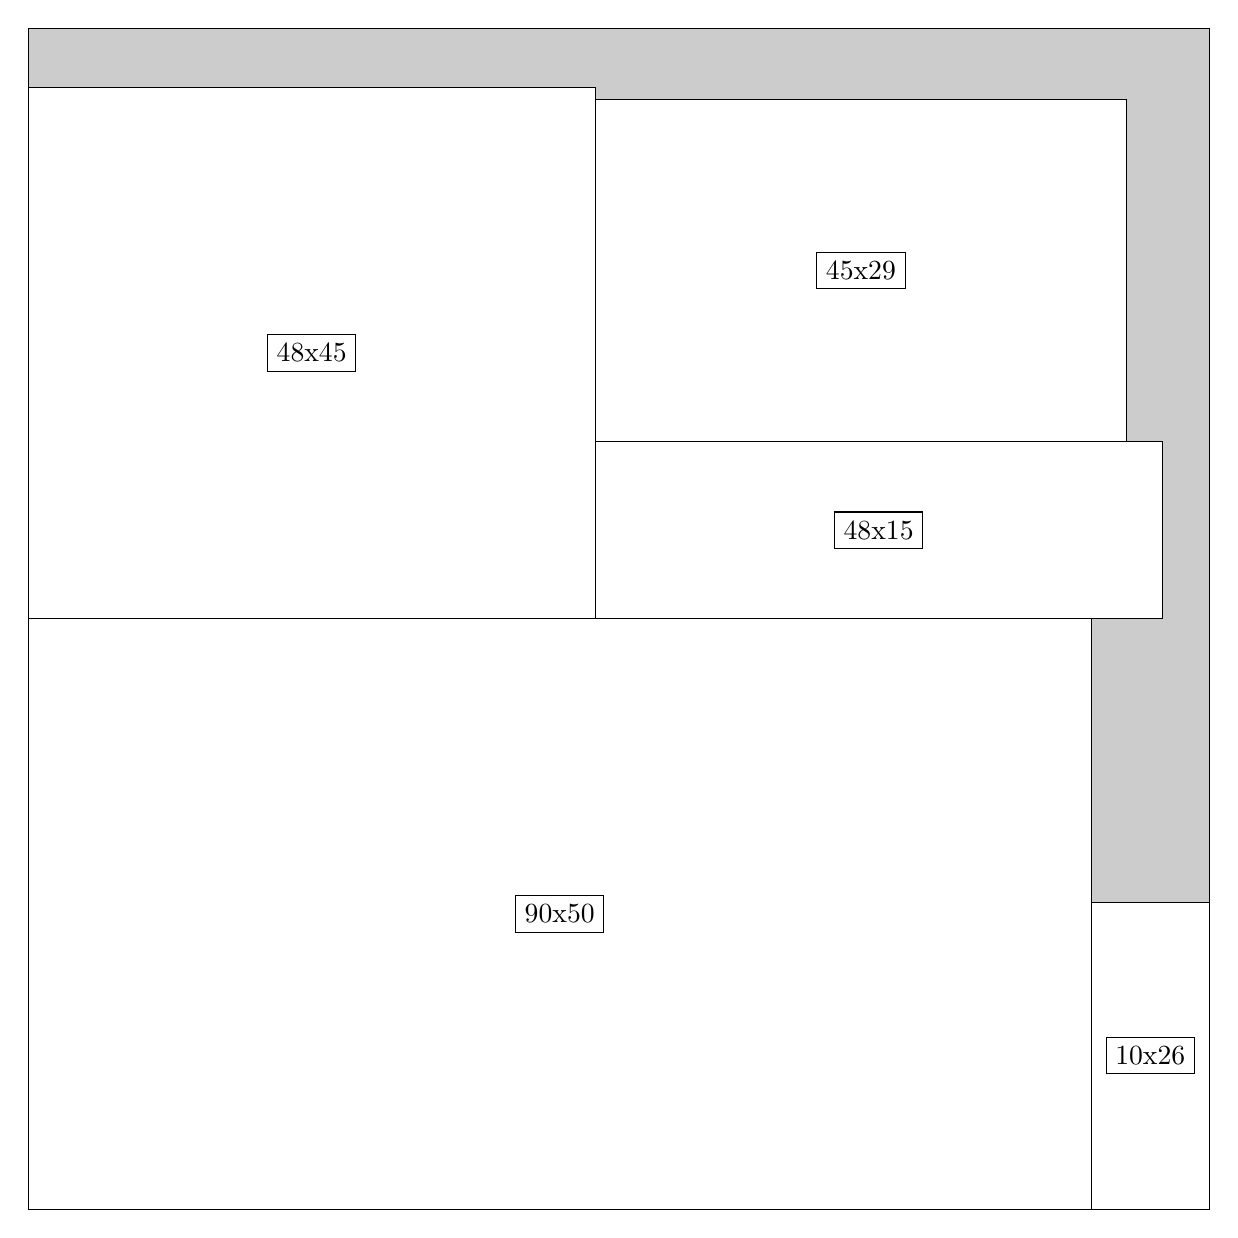
\begin{tikzpicture}[shorten >=1pt,scale=1.0,every node/.style={scale=1.0},->]
\tikzstyle{vertex}=[circle,fill=black!25,minimum size=14pt,inner sep=0pt]
\filldraw[fill=gray!40!white, draw=black] (0,0) rectangle (15.0,15.0);
\foreach \name/\x/\y/\w/\h in {90x50/0.0/0.0/13.5/7.5,48x45/0.0/7.5/7.199999999999999/6.75,45x29/7.199999999999999/9.75/6.75/4.35,48x15/7.199999999999999/7.5/7.199999999999999/2.25,10x26/13.5/0.0/1.5/3.9}
\filldraw[fill=white!40!white, draw=black] (\x,\y) rectangle node[draw] (\name) {\name} ++(\w,\h);
\end{tikzpicture}


w =90 , h =50 , x =0 , y =0 , v =4500
\par
w =48 , h =45 , x =0 , y =50 , v =2160
\par
w =45 , h =29 , x =48 , y =65 , v =1305
\par
w =48 , h =15 , x =48 , y =50 , v =720
\par
w =10 , h =26 , x =90 , y =0 , v =260
\par
\newpage


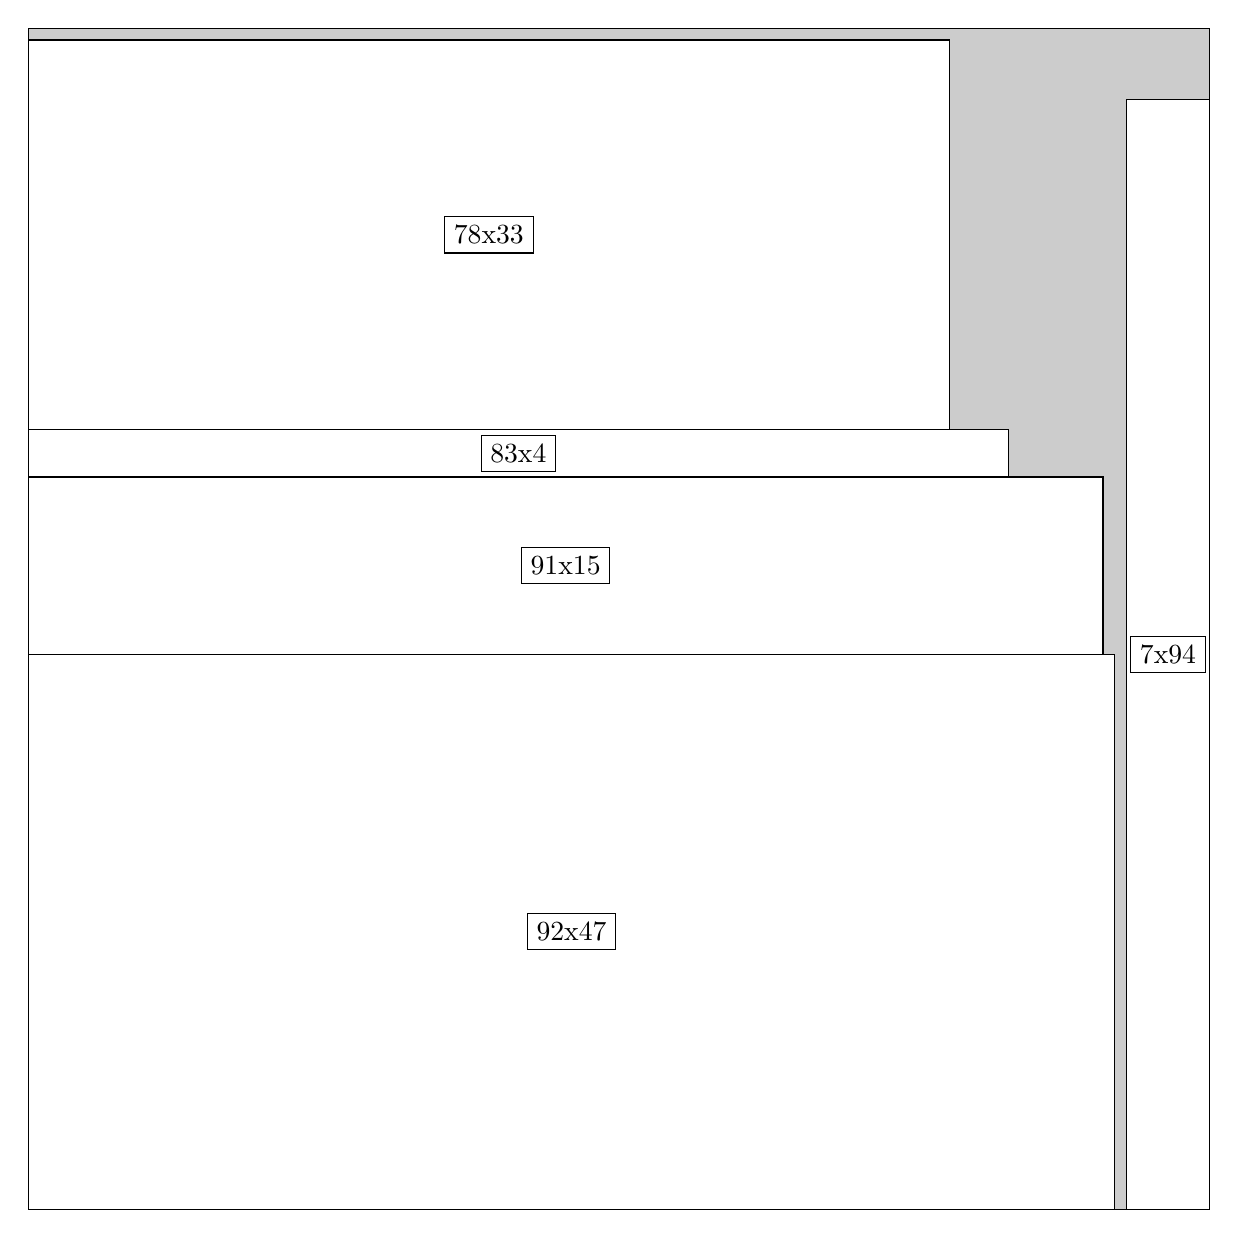
\begin{tikzpicture}[shorten >=1pt,scale=1.0,every node/.style={scale=1.0},->]
\tikzstyle{vertex}=[circle,fill=black!25,minimum size=14pt,inner sep=0pt]
\filldraw[fill=gray!40!white, draw=black] (0,0) rectangle (15.0,15.0);
\foreach \name/\x/\y/\w/\h in {92x47/0.0/0.0/13.799999999999999/7.05,78x33/0.0/9.9/11.7/4.95,91x15/0.0/7.05/13.65/2.25,7x94/13.95/0.0/1.05/14.1,83x4/0.0/9.299999999999999/12.45/0.6}
\filldraw[fill=white!40!white, draw=black] (\x,\y) rectangle node[draw] (\name) {\name} ++(\w,\h);
\end{tikzpicture}


w =92 , h =47 , x =0 , y =0 , v =4324
\par
w =78 , h =33 , x =0 , y =66 , v =2574
\par
w =91 , h =15 , x =0 , y =47 , v =1365
\par
w =7 , h =94 , x =93 , y =0 , v =658
\par
w =83 , h =4 , x =0 , y =62 , v =332
\par
\newpage


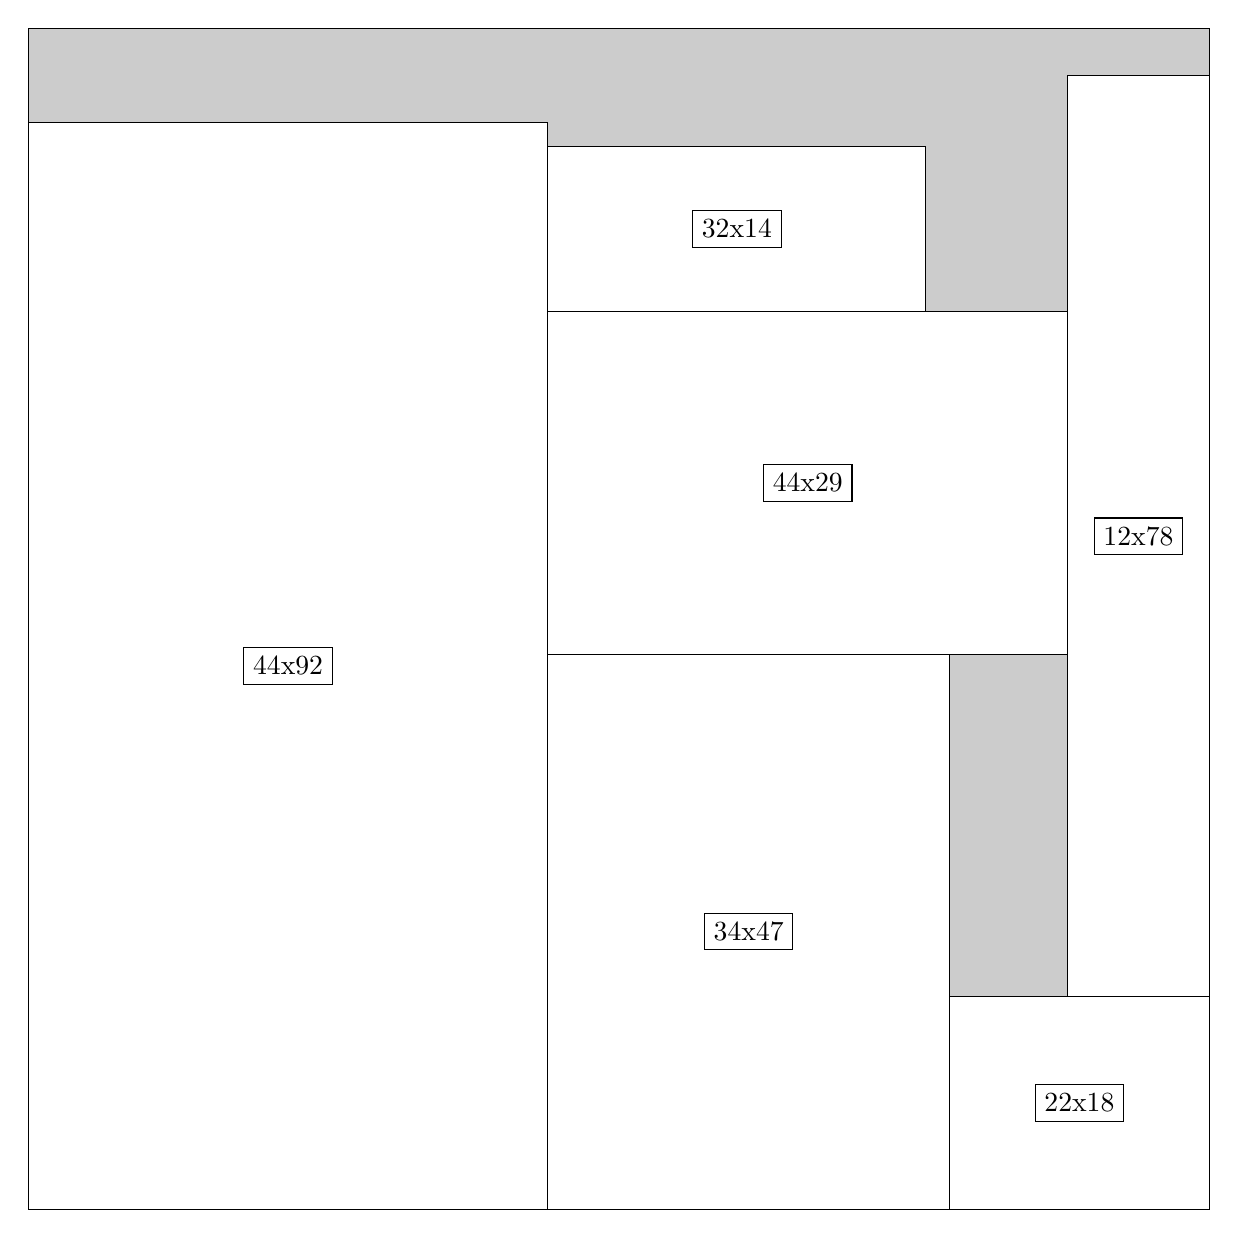
\begin{tikzpicture}[shorten >=1pt,scale=1.0,every node/.style={scale=1.0},->]
\tikzstyle{vertex}=[circle,fill=black!25,minimum size=14pt,inner sep=0pt]
\filldraw[fill=gray!40!white, draw=black] (0,0) rectangle (15.0,15.0);
\foreach \name/\x/\y/\w/\h in {44x92/0.0/0.0/6.6/13.799999999999999,34x47/6.6/0.0/5.1/7.05,44x29/6.6/7.05/6.6/4.35,12x78/13.2/2.6999999999999997/1.7999999999999998/11.7,32x14/6.6/11.4/4.8/2.1,22x18/11.7/0.0/3.3/2.6999999999999997}
\filldraw[fill=white!40!white, draw=black] (\x,\y) rectangle node[draw] (\name) {\name} ++(\w,\h);
\end{tikzpicture}


w =44 , h =92 , x =0 , y =0 , v =4048
\par
w =34 , h =47 , x =44 , y =0 , v =1598
\par
w =44 , h =29 , x =44 , y =47 , v =1276
\par
w =12 , h =78 , x =88 , y =18 , v =936
\par
w =32 , h =14 , x =44 , y =76 , v =448
\par
w =22 , h =18 , x =78 , y =0 , v =396
\par
\newpage


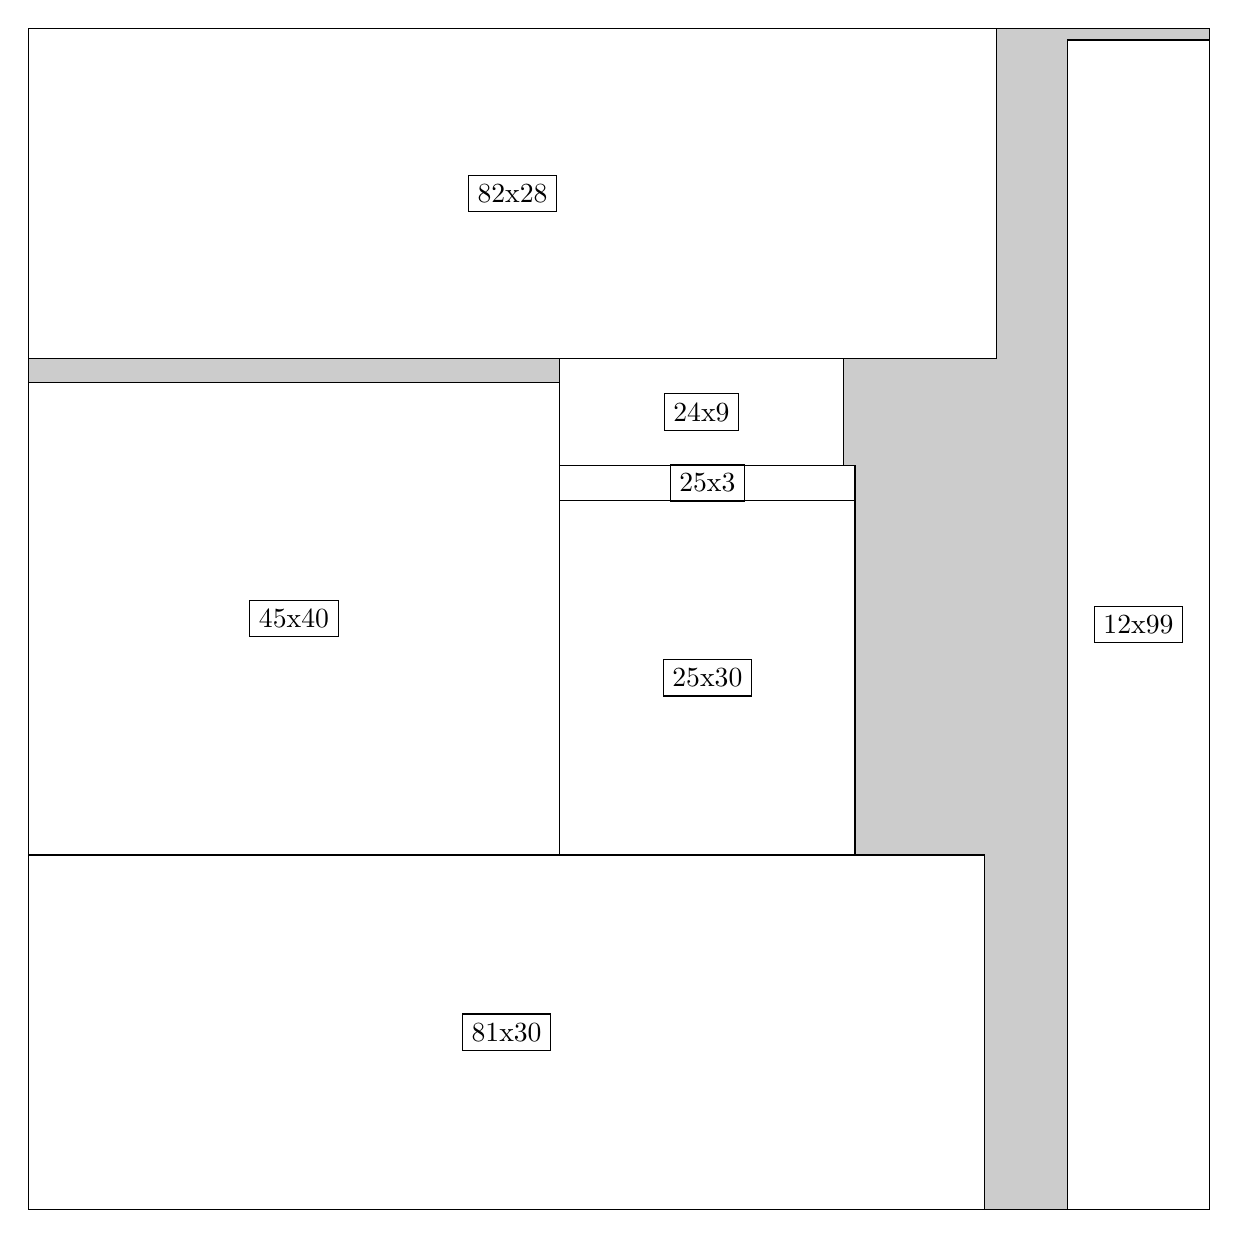
\begin{tikzpicture}[shorten >=1pt,scale=1.0,every node/.style={scale=1.0},->]
\tikzstyle{vertex}=[circle,fill=black!25,minimum size=14pt,inner sep=0pt]
\filldraw[fill=gray!40!white, draw=black] (0,0) rectangle (15.0,15.0);
\foreach \name/\x/\y/\w/\h in {12x99/13.2/0.0/1.7999999999999998/14.85,81x30/0.0/0.0/12.15/4.5,82x28/0.0/10.799999999999999/12.299999999999999/4.2,45x40/0.0/4.5/6.75/6.0,25x30/6.75/4.5/3.75/4.5,24x9/6.75/9.45/3.5999999999999996/1.3499999999999999,25x3/6.75/9.0/3.75/0.44999999999999996}
\filldraw[fill=white!40!white, draw=black] (\x,\y) rectangle node[draw] (\name) {\name} ++(\w,\h);
\end{tikzpicture}


w =12 , h =99 , x =88 , y =0 , v =1188
\par
w =81 , h =30 , x =0 , y =0 , v =2430
\par
w =82 , h =28 , x =0 , y =72 , v =2296
\par
w =45 , h =40 , x =0 , y =30 , v =1800
\par
w =25 , h =30 , x =45 , y =30 , v =750
\par
w =24 , h =9 , x =45 , y =63 , v =216
\par
w =25 , h =3 , x =45 , y =60 , v =75
\par
\newpage


\end{document}